\chapter{Literature Review}
\label{Literature Review}

To model the behaviour of rolling element bearings under conditions in electrified powertrains, component level models are required. At the core of these models is the dynamic bearing model.

Prior to the 1960’s, bearing studies were primarily conducted experimentally. Empirical formulations were derived to model their performance in early work by Stribeck \cite{Stribeck1907} and Lundberg and Palmgren \cite{Lundberg1952} \cite{Palmgren1959} amongst others. As computer technology improved post-1960, modelling theory and application grew rapidly, pioneered largely by the work of Jones \cite{Jones1960} and Harris \cite{Harris1984}. In the pursuit of highly efficient and reliable bearings, modelling and the need for accurate representation of the physical phenomena has become important. It is not possible to conduct experimental testing for the large array of design and operational parameters that bearings are required for, therefore experimentally validated numerical analysis is employed.

\subsection{Quasi-static Bearing Models}

Early models predicting load distribution in the rolling elements can calculate bearing stiffness and fatigue life with relative accuracy. These were primarily quasi-static and based on force equilibrium. Studies of static ball bearings under simple radial loading were performed by Stribeck \cite{Stribeck1907} and improved upon by Palmgren \cite{Palmgren1959} for the case of nominal internal clearance. Static models computing radial and axial loads based on a load distribution factor and the angular position of the roller were found using Sjovall’s integration model \cite{Sjovall1933}, however this was only applicable if the ratio of radial to axial loads is within a particular range. Rumbarger \cite{JRumbarger1962} developed a model using Sjovall’s integral method for purely axial loading of thrust bearings, capable of calculating moment load due to axial load eccentricity. 

It was the work of Jones \cite{Jones1960} and his general theory for load deflection analysis of bearings that extended the capability of these models. His work accounted for centrifugal and gyroscopic loading, and unlike previous models, the inner bearing race had 5 degrees of freedom (DOFs); three translational and two rotational displacements that correspond to the external forces in all three cartesian coordinates and moments applied about two. Bearing equilibrium is obtained at each rolling element by observing the load and corresponding motion of the elements. Jones also included the individual stiffness at the contact between rolling elements and raceways, using the Hertzian contact load-deflection relationship to obtain roller load based on contact deflection. This technique could be applied to both ball and roller bearings by varying the exponent of localised deflection. 

Jones' model was considerd limited due to the assumption that misalignment effects on the elements are negligible. Harris \cite{Harris1984} improved on it by introducing the slicing method along the length of the rollers. This enabled determination of the load distribution along the contact in roller bearings. This method, known as the Jones-Harris method, was then applicable for highly loaded conditions and able to compute misaligned cases. Vector and matrix methods to analytically solves the quasi-static problem based on the work of Jones and Harris were then presented for tapered roller bearing cases by Andréason \cite{Andreason1973} and Liu \cite{Liu1976}. de Mul et al. \cite{DeMul1989_2} developed a model for ball and roller bearing equilibrium and stiffness matrix calculations which has the advantage of having load-deflection equations in matrix form, therefore implementation of this model is simpler.

Additional functionality has been added to these models such as the effects of thermal expansion on the load-deflection analysis \cite{Jorgensen1997}. Numerical models for heat generation based on frictional torque and 3-dimensional transfer through contacting elements was used to account for the expansion. It was found that expansion increased the bearing stiffness and thus natural frequency of the shaft-spindle system due to greater interference of the roller race contact. The authors also investigated the effect of ring expansion due to centrifugal force at high speeds \cite{Jorgensen1998} and found that natural frequency of the spindle decreased at higher rotational speeds – of particular note for high speed automotive applications.

\subsection{Contact Load and Deflection Calculation}

The contact between rolling elements and raceways and the subsequent load and deformation generated at this contact is regarded as one of the most important issues in rolling-element bearing modelling. For a ball bearing, classical Hertzian theory is used to calculate the load-deformation relationship. However, the line contact is more complex.

There exist three methods to determine this relationship for the line contact in roller bearings: the slicing technique, 3D contact method and the alternative slicing technique. The slicing technique \cite{Andreason1973} divides the roller-race contact region into a finite number of slices, with the total contact forces calculated from the summation of forces of each individual slice. Various formulae have been developed to perform this calculation, all yielding very similar results. A drawback of this method is that the load on each slice does not influence the surrounding slices as they are treated independently. This means that pressure concentrations such as edge stresses on the contact are not captured. The 3D contact method uses the Boussinesq half-space force-displacement relationships and flexibility method of structural analysis. The contact pressure distribution and normal approach between the bodies is found using an iterative scheme, making this a time-consuming method. Kabus et al. \cite{Kabus2012} addressed this in their 6-dof quasi-static time-domain bearing model  by pre-processing a series of contacts at different centreline approaches  and roller tilt angles, then interpolating these results in the actual simulations. This negated the need to solve the iterative scheme at each time step. This allowed for bearing misalignment, roller centrifugal forces, flange contact and roller tilt moments to be analysed. 

Teutsch and Sauer \cite{Teutsch2004} improved on the slicing technique with their alternative slicing method. Using a matrix of weighted influence coefficients, the effects of force on the deflection of neighbouring slices was captured. It is not too dissimilar in concept to the 3D contact method but with improved computation times. de Mul et al. \cite{DeMul1989_2} compared the slicing technique with their more complex non-Hertzian model and concluded that the simplicity and accuracy of the slicing method yielded accurate and faster results. Harris and Kotzalas \cite{Harris2007} also concluded that the slicing technique, whilst unable to reflect edge stress concentrations, provides a suitably accurate load-displacement result as stresses are only distributed over a small area. For the purpose of load equilibrium, these stresses can be neglected. Misalignment or loading on roller ends is not captured using this technique, therefore for fatigue life estimates this may produce non-conservative results; for this, the approach by Kabus et al. should be used. In general, the slicing technique is the most widely used, owing to its simplicity, speed, and sufficient accuracy.

\subsection{Dynamic Bearing Models}

Quasi-static bearing models that solve force equilibrium within the bearing are only applicable under steady state operating conditions. Transient operating conditions such as acceleration or deceleration of the bearing requires dynamic modelling, particularly important for high-speed applications. In dynamic bearing models, a system of differential equations based on Newton’s second law of motion are used. This allows for a time-varying input force such as eccentric rotor unbalances or fluctuating loading conditions present in transmissions. Static equilibrium solutions such as those presented are used within these models to calculate load-deflection and individual element loading. 

Hitherto, a multitude of models predicting bearing dynamics have been posed for roller bearings. These investigate the dynamic effect of geometrical and topographical parameters such as surface waviness, surface defects, and the variable compliance affect. This variable compliance effect is caused by time-varying stiffness variations off the inner and outer race bearing contact as rollers change their orbital position and pass through the loaded region. Even with perfect bearing geometry free from any defects, vibration will still occur due to this \cite{Sopanen2003_1}.
  
Simplified 2 degree of freedom models \cite{Walters1971} consider purely in-plane motion of rolling elements in the radial and lateral directions of the bearings for investigation of frequency response to defects \cite{Meyer1980} and the varying compliance effect \cite{Sunnersjo1978}.  Time varying forces on cutting tool spindles and the effects on radial loading assuming no axial thrust loads or vibration can also be investigated in 2 DOF \cite{Matsubara1988}. These models increase in complexity up to 5-DOF  to observe moment loading and centrifugal effects \cite{Rahnejat2004} \cite{Gupta1979}. Most of these models assume the bearing rollers and races are rigid bodies. All these analyses also assume a dry contact between rolling elements and races which was assumed valid under the elastohydrodynamic regime of lubrication. The fluid film behaves as an amorphous, incompressible solid and generated pressures conform closely to a Hertzian distribution in the loaded region. This, however, neglects the effect of the lubricant film thickness in the contact mechanics and thus underestimates the contact deflection and hence load. Furthermore, the assumption of rigid rollers and races which is widely used amongst bearing dynamic models to simplify the computation is often not representative of the physical phenomena of modern shaft-bearing systems.

\subsection{Lubricated Dynamic Bearing Models}

To fully numerically analyse a complement of rolling elements at each step of dynamic analysis, accounting for lubricant film thickness at the contact, is a time-consuming limitation. Historically the analysis of rolling element bearings has been decoupled into two stages. The first stage is a classic dry Hertzian-contact analysis of the roller-raceway contact due to the cyclic variation in geometric bearing centre \cite{Aini1990}. The displacement of the bearing centre is obtained through solving equations of motion and roller load is obtained using the Hertzian load-deflection relationship. Extrapolated film thickness equations use the transient load yielded from dry analysis in a second stage study to find central film thickness. This approach does not implicitly consider the effect of the lubricant film on the prevailing bearing motion and load, which is hence underestimated. To overcome these shortcomings, quasi-static analyses employing film thickness formulae in conjunction with Hertzian contact mechanics are required.

Rahnejat and Gohar \cite{Rahnejat1985} employed these formulae to account for film thickness on the load share of an individual roller within the bearing complement. This coupled a two-dimensional dynamic model for a radial deep groove ball bearing with extrapolated film formulae implicitly. More reasonable bearing vibration amplitudes resulted than de-coupled analyses which were only suitable for spectral contributions and unable to produce accurate magnitudes. This work was later extended to a 5-dof model by Aini et al. \cite{Aini2002} which included axial thrust effects and moment loading in a shaft-bearing system. The analytical film thickness formulae used do not offer the capabilities of a full numerical solution such as the modelling of inlet starvation at high speeds. They do, however, offer a much faster solution when implicitly coupled with dynamic bearing analysis.

Film shape and the elastohydrodynamic pressure profile at the contact could not be calculated in these studies, preventing more detailed analysis such as thermal and sub-surface stress analysis. To determine tribological contact conditions, Mohammadpour et al. \cite{Mohammadpour2015c} utilised a full numerical elastohydrodynamic analysis explicitly. Load values on an individual roller at each instantaneous position of the orbit were obtained from the implicit tribodynamic analysis and used within the numerical model. The stiffness and damping of the EHL film is neglected due to its rigid-like stiffness which is several orders of magnitude higher that the Hertzian contact \cite{Dareing1975} \cite{Mehdigoli1990}. 

These lubricated dynamic models were performed for low shaft rotational speed. In Mohammadpour’s analysis, input shaft speeds of 209 rad/s resulted in much slower entrainment velocities than in EV case studies. The rollers and races were also considered rigid in these investigations. Thus far, tribo-dynamic models have not been found that model the bearing races as flexible bodies or at high speeds.

\subsection{Hertzian Contact Mechanics}

Two types of contacts occur in machine elements: conformal and non-conformal. Conformal contacts occur between a concave and a convex body of similar radius, such as in journal bearings. This leads to a relatively large contact area over which load can be distributed and resultant pressures are in the order of MPa. The contact between rolling elements and races is non-conformal in nature as the contacting surfaces are both convex. This type of contact creates a very small contact region over which force is transmitted, leading to very high contact pressures being generated in the order of GPa. Under these pressures, the contact surfaces deform elastically. In the case of a lubricated contact, a lubricant film forms in between the contacting surfaces in the order of microns (typically < $2 \mu \mathrm{m}$) \cite{Gohar2018}. Non-conformal contacts are typically found in rolling element bearings, gear contacts and cam follower pairs.

A fundamental aspect of these contacts is that the approach of the bodies under external load leads to the deformation of both bodies and the emergence of a contact patch. For two cylinders in contact with their axes parallel, a rectangular or line contact is formed along the length of the cylinders with width $2b$ (see Figure \ref{LineContact}). An elliptical point contact results from contacting bodies that have different radii along both principal axes \cite{Johnson1985} (see Figure \ref{PointContact}). In the case of cylindrical elements, such as those in NRBs, CRBs and TRBs, the mutual approach of the roller and race forms a line contact. Spherical elements, such as those found in DGBBs and ACBBs, generate an elliptical contact at their conjunction with the raceway

\begin{figure}
	\centerline{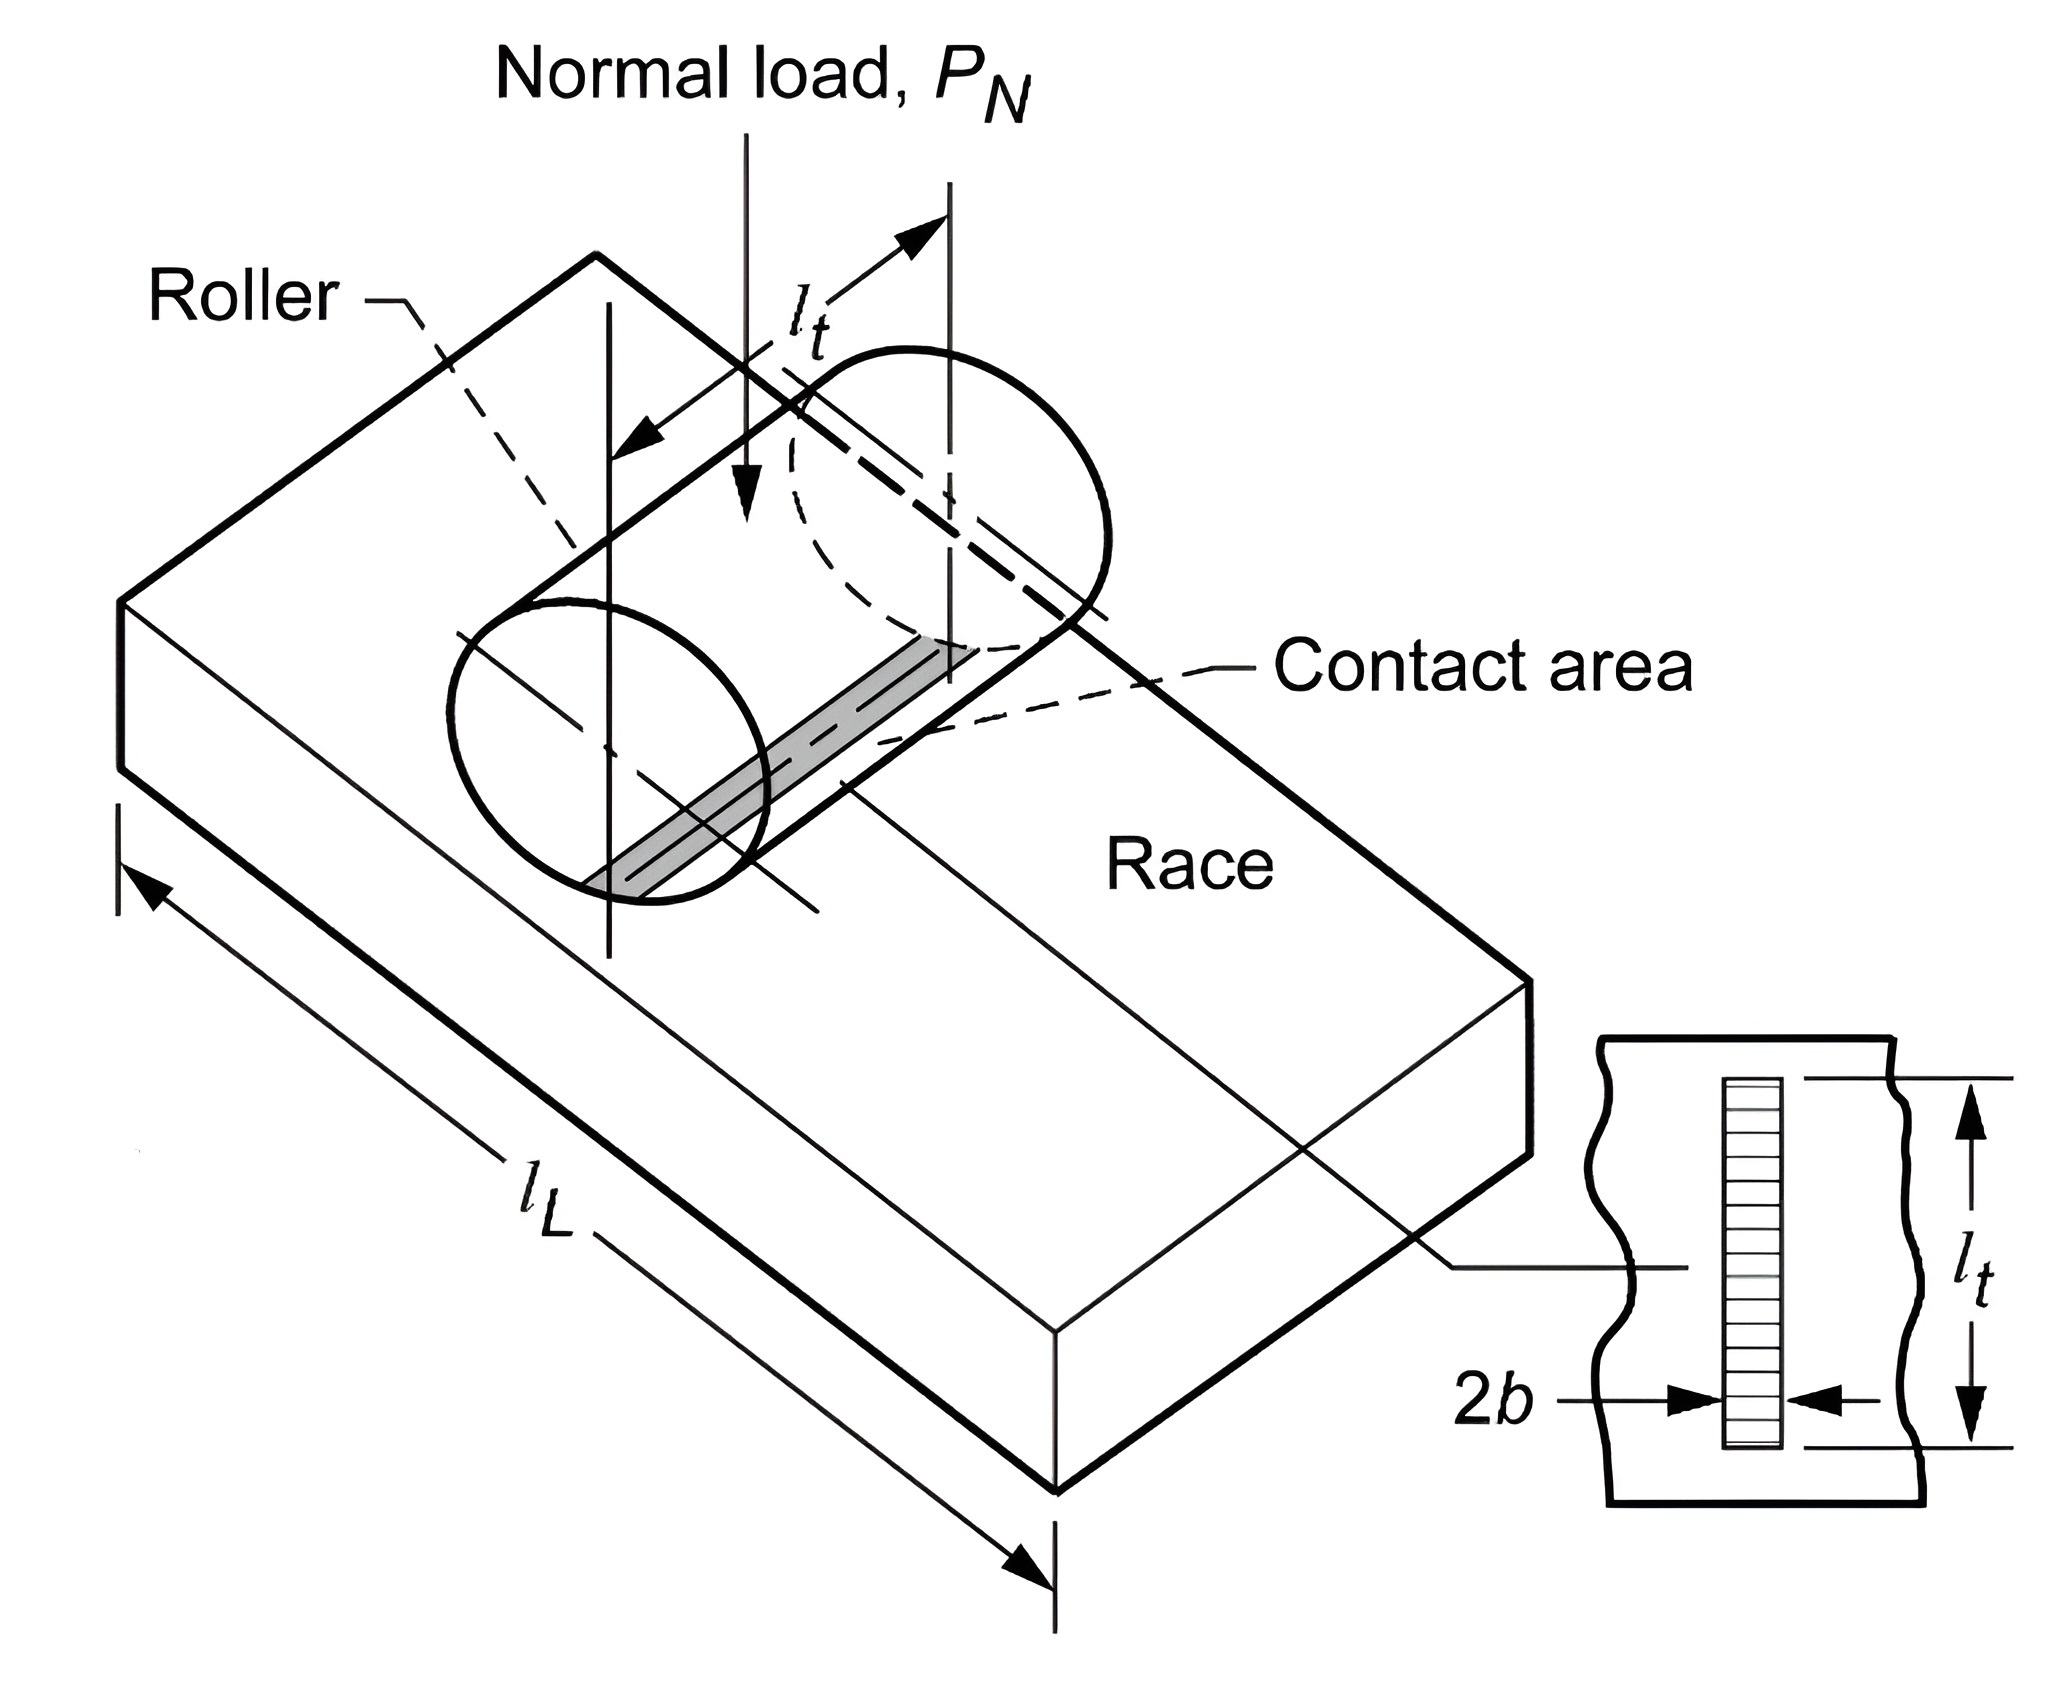
\includegraphics[width=125 mm]{LineContact.png}}
	\caption{Roller-race model for line contact \cite{Zaretsky2016}}
	\label{LineContact}
\end{figure}

\begin{figure}
	\centerline{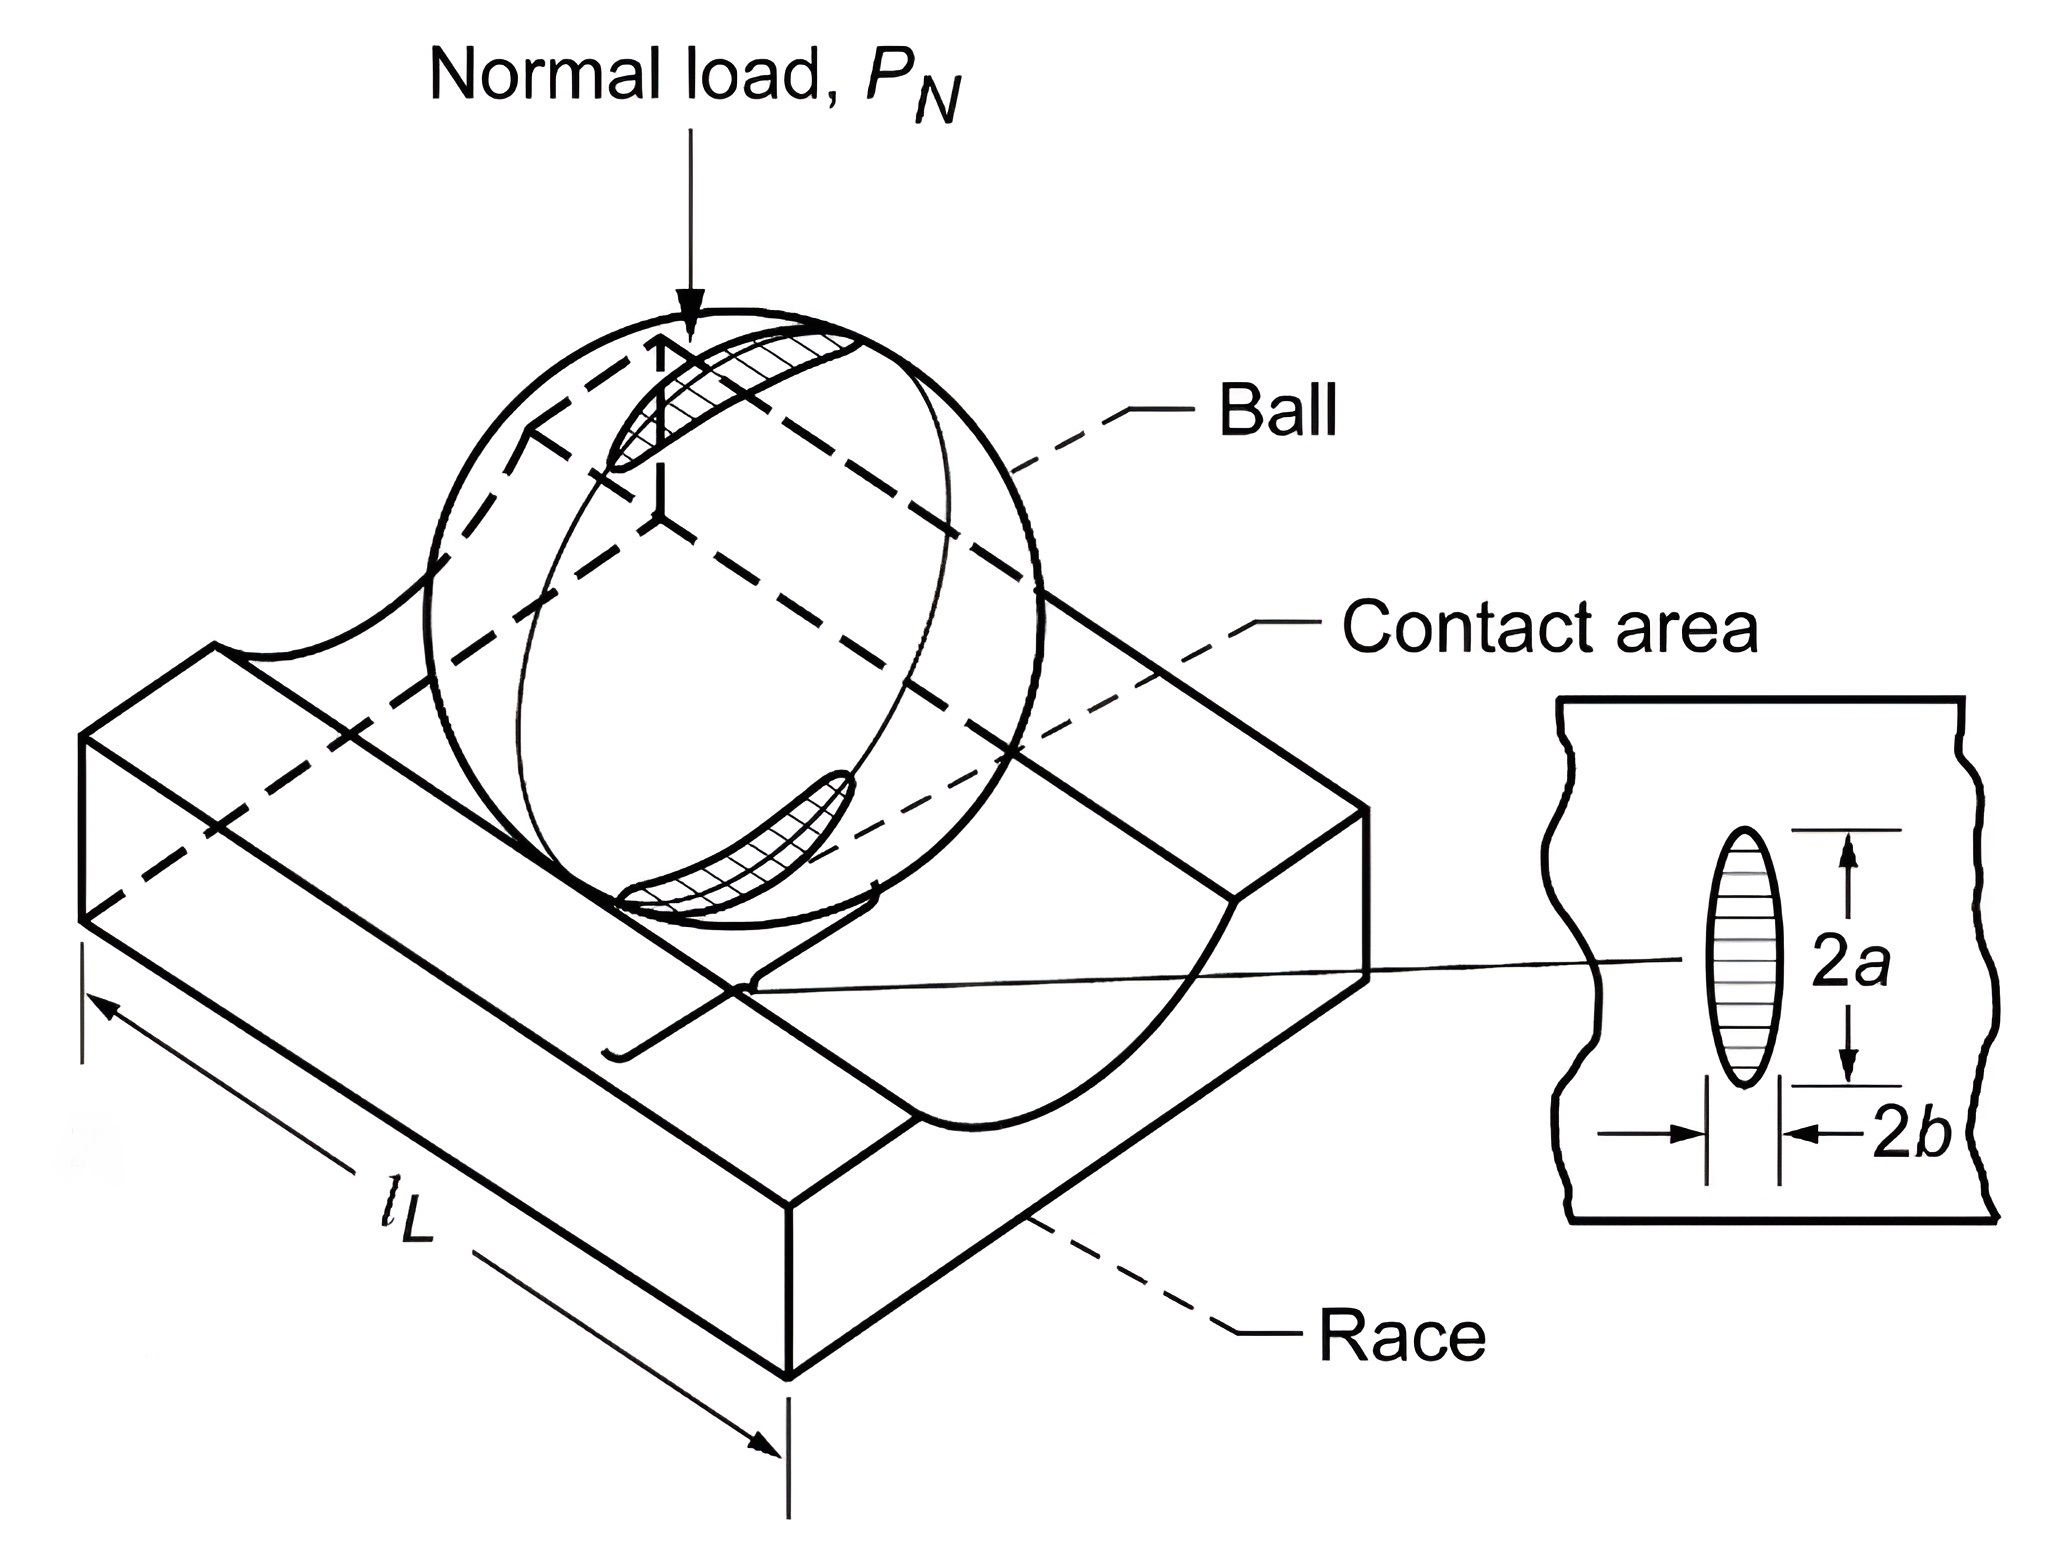
\includegraphics[width=125 mm]{PointContact.png}}
	\caption{Ball-race model for point contact \cite{Zaretsky2016}}
	\label{PointContact}
\end{figure}

Two cylinders with radii $R_1$ and $R_2$ contacting in a non-conformal manner can be simplified as a rigid cylinder in contact with an elastic half-space. This cylinder, as represented in Figure \ref{LineContact}, has a radius known as the reduced radius, $R^{\prime}$:

\begin{equation}\label{eq2.1}
	\frac{1}{R^{\prime}}=\frac{1}{R_1}+\frac{1}{R_2}
\end{equation}

The material properties of the two bodies are evaluated in a similar way. The elastic modulus, $E$ and Poisson's ratio, $v$, of both bodies are combined to calculate the reduced elastic modulus:

\begin{equation}\label{eq2.2}
	\frac{1}{E^{\prime}}=\frac{1}{2}\left(\frac{1-v_1^2}{E_1}+\frac{1-v_2^2}{E_2}\right)
\end{equation}

According to Hertz's theory of elastostatic solids in contact \cite{Hertz1881}, assuming the contact is frictionless, when load is applied to the cylinder it will experience very small strains. The amount that the cylinder deflects is much smaller than the radius of the cylinder, that is $\delta \ll R^{\prime}$. The total area of the contact is also much smaller than the radius of the cylinder $a \ll R^{\prime}$ (exaggerated in \ref{HertzianContactDeflection}). For example, a cylinder with a radius in order of $mm$ will have a contact width of a few tenths of a $mm$ and deflection a few tenths of a micron ( $\delta<a \ll$ $\left.R^{\prime}\right)$.

\begin{figure}
	\centerline{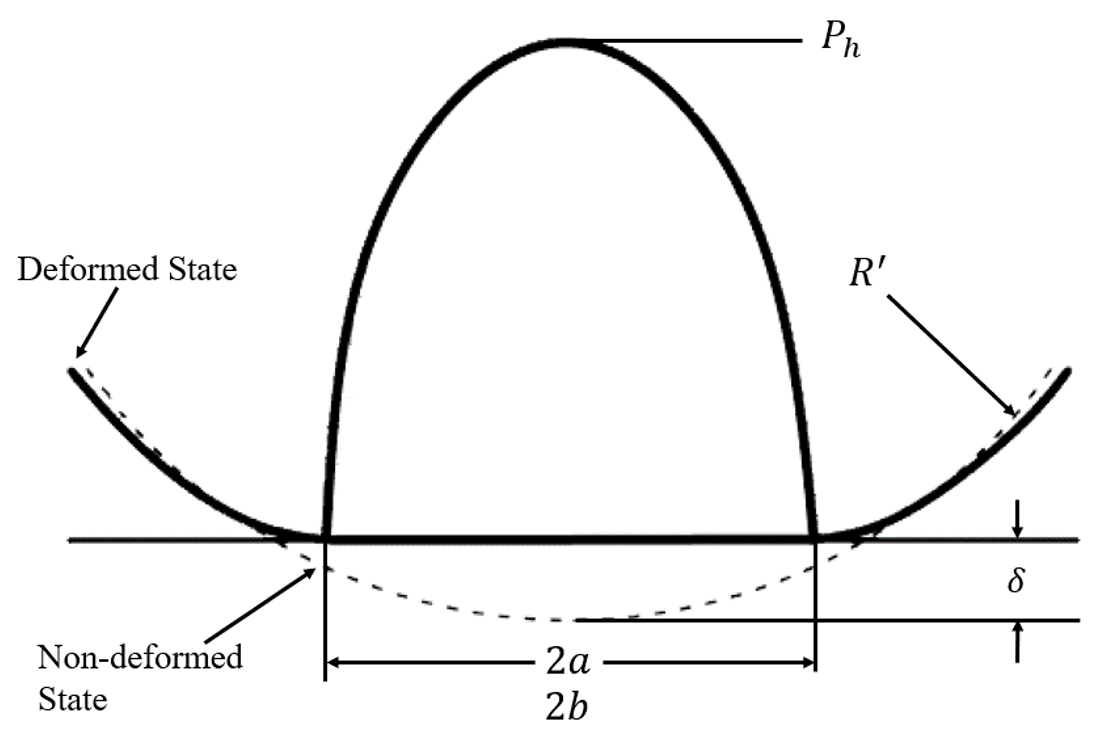
\includegraphics[width=100 mm]{Hertzian_Contact_Deflection.png}}
	\caption{Hertzian Contact Deflection}
	\label{HertzianContactDeflection}
\end{figure}

The value of the deflection determines the stiffness of the contact and the displacement of the inner bearing race with respect to the outer. The contact area determines the contact pressures and hence maximum sub-surface stresses. Excessive sub-surface stress could lead to inelastic deformation and subsequent fatigue spalling.

Analytical formulae provide a way of calculating the dimensions of the contact patch, $b$, and the resultant maximum Hertzian pressure, $P_h$ given a known force, $w$, material properties and geometry of bodies. For the case of the line contact these are:

\begin{equation}\label{eq2.3}
	b=\sqrt{\frac{8 w R_{z x}}{\pi E_r}}
\end{equation}

\begin{equation}\label{eq2.4}
	P_h=\sqrt{\frac{2 w}{\pi b}}
\end{equation}

where $w$ is load per unit length.

\subsection{Elastohydrodynamic Lubrication}

Under the EHL regime, both the elastic deformation of the solids in contacts as well as hydrodynamic theory are considered. Elastic bodies in contact for the case of ellipsoidal contacts was first investigated by Hertz in 1881 [6], allowing him to obtain the pressure distribution within an ellipsoidal contact. Separate studies on hydrodynamic lubrication were being performed by Reynolds in 1886 [7], based on a simplified version of the Navier-Stokes equation. It took a further 30 years before the two studies would be combined.

Early EHL studies began in 1916 when the pioneering work by Reynolds was applied to a simplified model of a gear-tooth contact by Martin [8]; replicated as two contacting cylinders. This analysis assumed that the solid bodies were rigid and the lubricant to behave with constant viscosity (ie. a hydrodynamic analysis). The resultant pressures were too high and the film thickness so low (1-10nm) that coverage of asperities (typical order of 100nm for machined gear teeth) was not possible. This contradicted experimental findings where machining tracks on high-speed gear tooth flanks were still visible after prolonged usage, which could only be explained by the presence of a sufficient lubricant film.

Between the 1930’s and 1950’s, significant research was performed to include both the elastic deformation of the surfaces and the effect of pressure on viscosity. Peppler [9] and Meldahl [10] both included the effects of surface deformation for non-conformal contacts, with Gatcombe [11] amongst others investigating viscosity increase due to the high pressure in the contact area. Typical EHL pressures are in the range of 0.5-4GPa and the resulting piezo-viscous properties were found to be partially instrumental to forming the film.

Considered the origin of EHL, Grubin’s pioneering work in 1949 [12] combined both elastic deformation and viscosity increase under pressure in film thickness calculations for the first time. In this analysis, he assumed that the deformed surface profiles in a highly loaded lubricated contact matched those produced in a classic dry Hertzian contact of the same materials and loading conditions. Reynolds equation could then be solved at the inlet region of the contact and a more accurate determination of the separation of the solids in the central region was found. This led to a film thickness in the predicted range (an order higher than Martin’s theory) and a more realistic pressure distribution than previous work. This pioneering study formed the basis for future EHL studies.

The first numerical solution of the line contact problem was presented shortly after by Petrusevich [13] which agreed with Grubin’s main conclusions. It contained the three main features of an EHL contact: a nearly parallel film in the contact zone with local constriction at the exit, a Hertzian pressure profile, and secondary local maximum pressure or ‘spike’ at the outlet (see Figure 6). In 1959, Dowson and Higginson [14] presented their numerical solution to the isothermal line contact EHL problem. Their iterative inverse method enabled the evaluation of film thickness and pressure distribution for line contact problems for lightly loaded cases. Throughout the 1960s, the authors investigated the effects of variables such as dimensionless surface velocity, materials parameter and load on EHL solutions. The authors then curve fitted their results and generated an empirical formula for isothermal line contacts [15], which was then improved upon by Dowson [16] and Dowson and Toyoda [17]. The formulae predict the minimum film thickness as a function of the rolling velocity, load and material parameters.

Empirical formulae are widely used today for analytical calculations that do not require the computational intensity of a full numerical solution. They are, however, somewhat limited to the operating parameters used in original simulations and do not offer the capabilities of a full numerical solution such as the modelling of inlet starvation at high speeds.